\documentclass[../tech_report_1.tex]{subfiles}
\graphicspath{{img/}{../img/}}
\begin{document}

% TODO: input results

\section{Shape L'Ane Rouge results}

There were fairly promising results for our multiresolution extension of the Shape L'Ane Rouge paradigm. We first validated the approach visually by choosing particular lambda values and reconstructing the shape using the permutation created from linear assignment.

\begin{figure}[ht]
	\caption{Shape L'Ane Rouge warping over several lambda}
	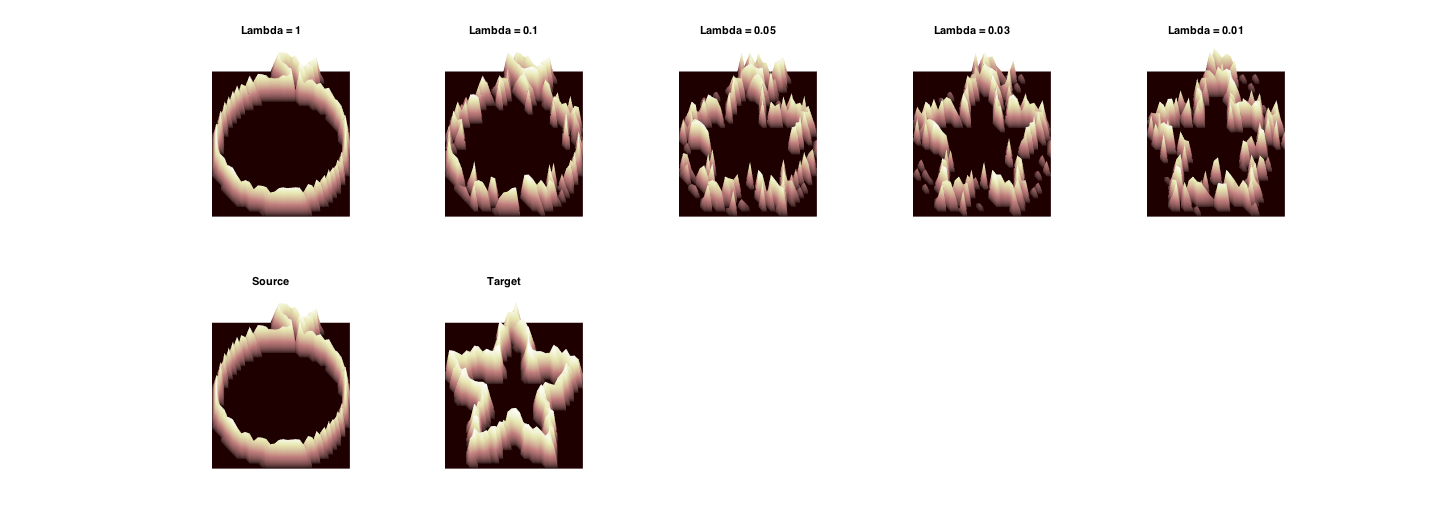
\includegraphics[width=\textwidth]{warp}
\end{figure}

Then we validated on the MPEG7 dataset. Our actual retrieval results weren't as high as we were hoping, which may be due to implementation details such as optimization of the lambda parameter. Improvement on retrieval results were negligible to negative.

\begin{figure}[ht]
\caption{MPEG7 retrieval results with linear assignment\label{fig:mpeg7_linassgn}}
\centering
\begin{tabular}{ l | l c r r}
	$\lambda$ values & No lin. assgn. & $\lambda=0.036$ & $\lambda=$1e-6 & $\lambda=$ 1e-8\\
	\hline
	Accuracy (bullseye metric)& 80.2\% & 80.0\% & 70.9\% & 73.2\% \\
\end{tabular}
\end{figure}

\end{document}